%===============================================================================
\section{Get the EE-UQ application}
%===============================================================================

\subsection{Download the application files}
%===============================================================================

SimCenter applications are available at the \href{https://simcenter.designsafe-ci.org/research-tools/overview/}{SimCenter website} under \emph{Research Tools}. Navigate to EE-UQ and click on \emph{Download App \& User Manual} to arrive at the download page (\autoref{fig:app_website}). There are at least four files available for download (\autoref{fig:app_choose_file}):

\begin{itemize}
    \item The PDF file is the User Manual that you are reading now.
    \item The MOV file is an video that provides an introduction to the usage of the application.
    \item The ZIP file is an archive that contains the application files for a Windows operating system.
    \item The DMG file is an archive that contains the application files for a Mac OS X operating system.
\end{itemize}

Click on the file that suits the operating system you use, and click on the Download button in the pop-up window to download it. On Windows, we recommend you to create a \texttt{C:/SimCenter/EE-UQ} directory and extract the contents of the \texttt{ZIP} archive there. On Mac, we recommend you to put the \texttt{DMG} archive in your Documents folder.

\begin{figure}[!htbp]
  \centering {
    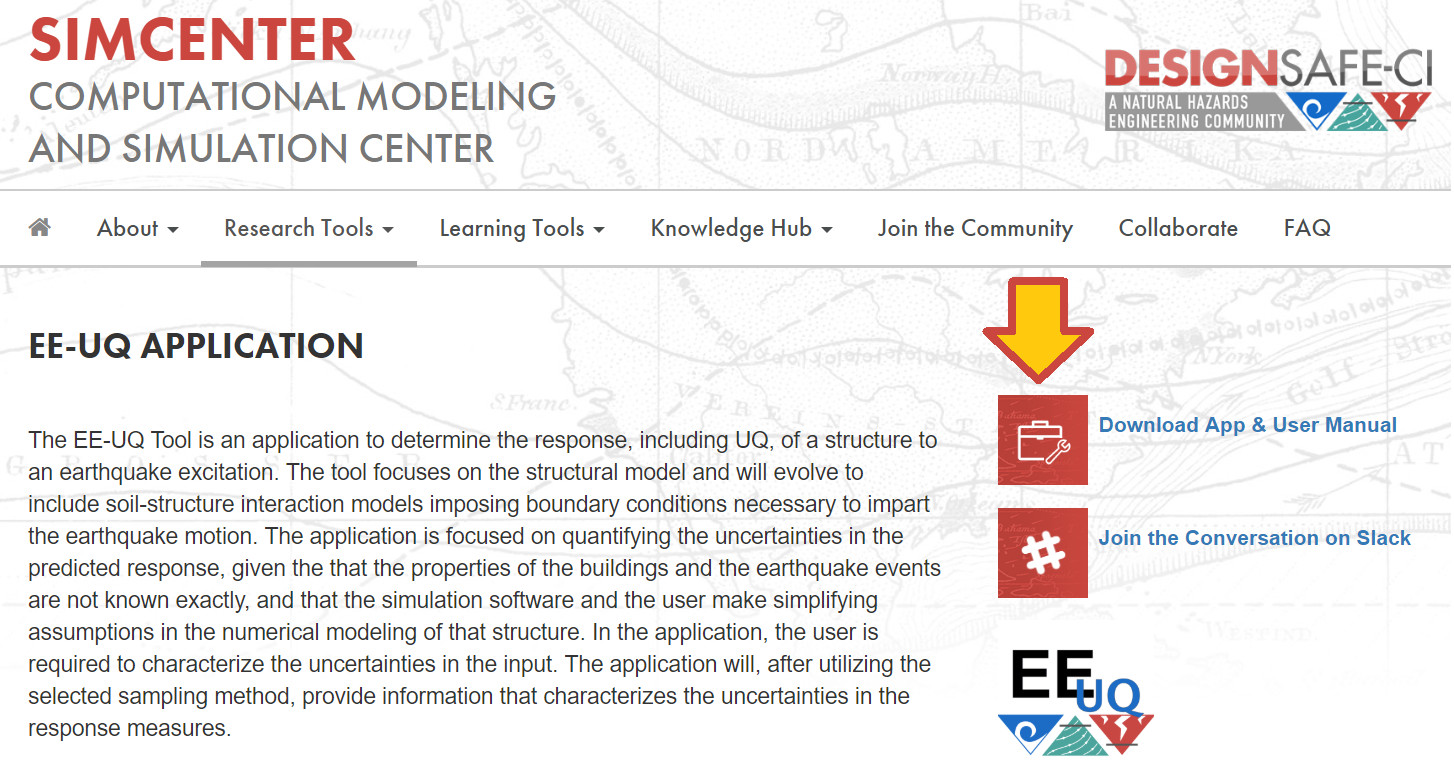
\includegraphics[width=0.8\textwidth]
    {figs/install/EE-UQ_app_website.png} }
  \caption{Download the EE-UQ application from the SimCenter website.}
  \label{fig:app_website}
\end{figure}

\begin{figure}[!htbp]
  \centering {
    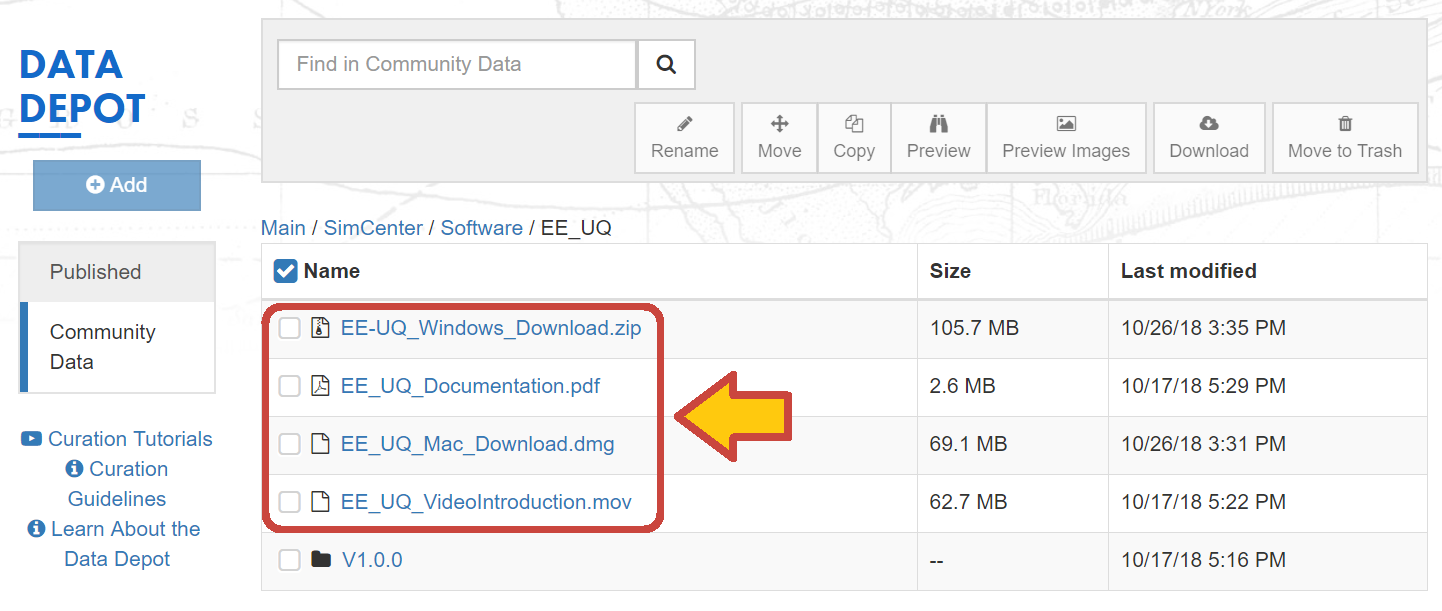
\includegraphics[width=0.8\textwidth]
    {figs/install/EE-UQ_app_choose_file.png} }
  \caption{Choose the appropriate file for your operating system.}
  \label{fig:app_choose_file}
\end{figure}

\subsection{Test the application}
%===============================================================================

On Windows, navigate to the \texttt{C:/SimCenter/EE-UQ} directory and run the \texttt{EE-UQ.exe} file. You should see the user interface (\autoref{fig:app_UI}) on your screen after starting the application.

On Mac, navigate to the \texttt{DMG} file in your Documents folder. Double-click on the file and its contents until you reach the \texttt{Contents/MacOS/} folder where you will find the EE-UQ executable. Drag and drop the executable to a Terminal window to start the application. You should see the user interface (\autoref{fig:app_UI}) on your screen after starting the application.

Note: The SimCenter is not recognized as either a Windows or an Apple vendor. Our applications are not recognized by the operating system as being signed. Consequently, you will receive a warning message when you start the EE-UQ application for the first time.

Note: The EE-UQ application requires additional software to work properly. Although the user interface loads, you will not be able to run calculations before installing those software.

\begin{figure}[!htbp]
  \centering {
    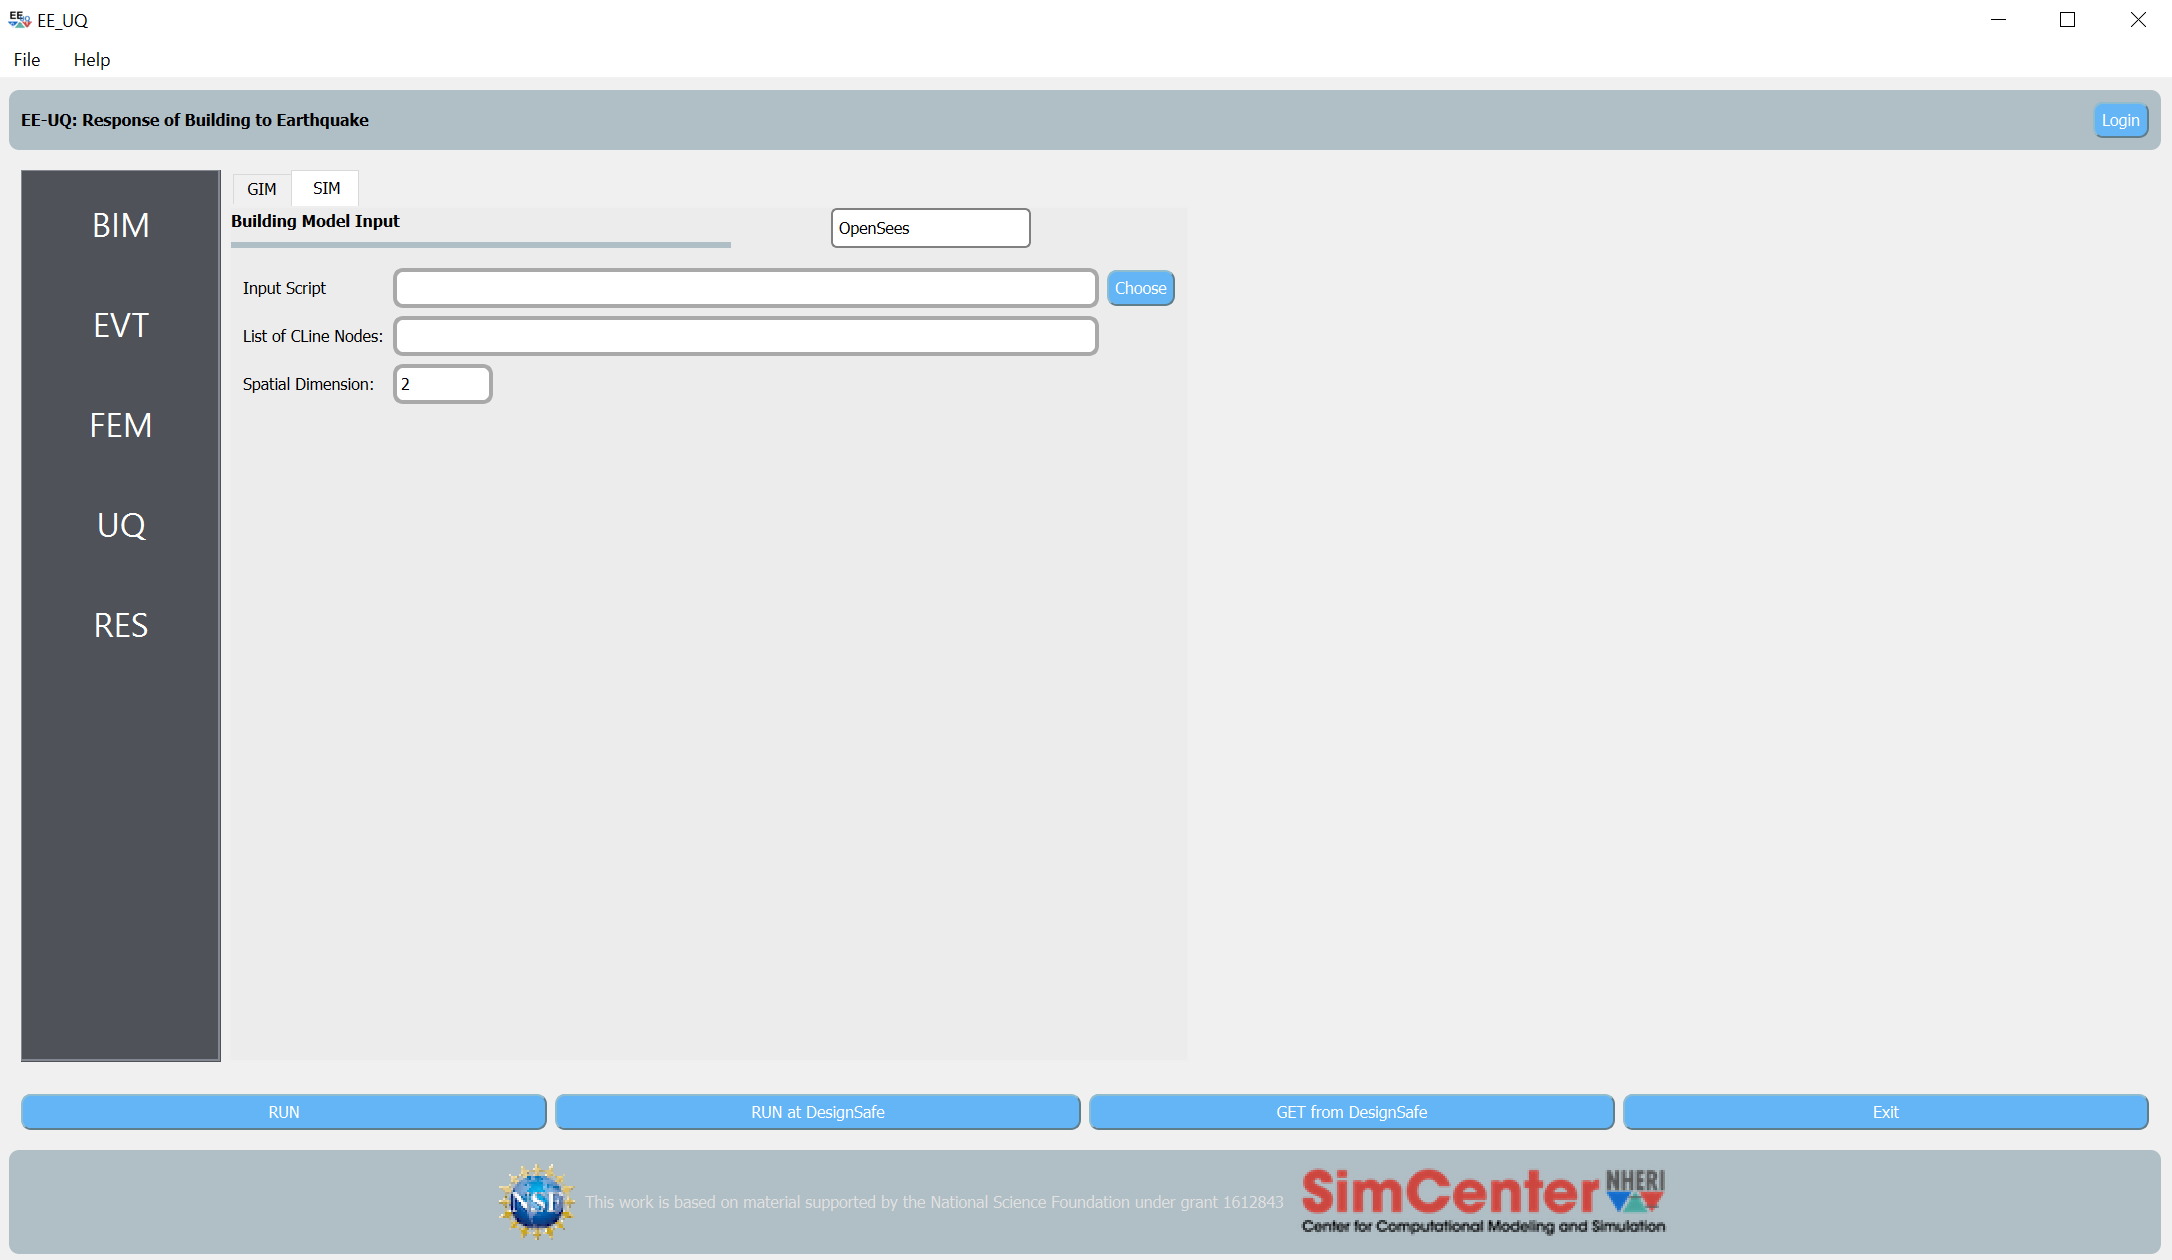
\includegraphics[width=0.8\textwidth]
    {figs/install/EE-UQ_app_UI.png} }
  \caption{The EE-UQ user interface after loading the application.}
  \label{fig:app_UI}
\end{figure}

%===============================================================================
\section{Set up your Python environment}
%===============================================================================

The SimCenter workflows are managed by Python scripts. These are required to perpare the input data for running analyses remotely on DesignSafe and also required for running analyses locally. 

\subsection{Install Python}

If you do not have a Python installation yet, we recommend installing \href{http://www.anaconda.com/distribution/#download-section}{Anaconda}. Anaconda provides all the important scientific packages in a single convenient install. We recommend installing the 64-Bit version based on Python 3.5 or newer.

Note: If you already have a Python installation that is Python 2.7 or newer, you do not have to install Anaconda to work with SimCenter applications.

If you prefer to install the standard Python distribution only, or you already have your own Python environment, please make sure that you also have the following packages available: \texttt{numpy}, \texttt{scipy}, \texttt{pandas}.

\subsection{Test Python}
%===============================================================================

Test if the python environment is set up properly by executing \texttt{python} in a terminal window. After Python starts, test if the packages are installed by executing \texttt{import numpy}, \texttt{import scipy}, and \texttt{import pandas}. You will receive an error message if a pacakage is missing. If no error appears, the terminal should look similar to \autoref{fig:python_test}. Exit Python by executing the \texttt{exit()} command.

\begin{figure}[!htbp]
  \centering {
    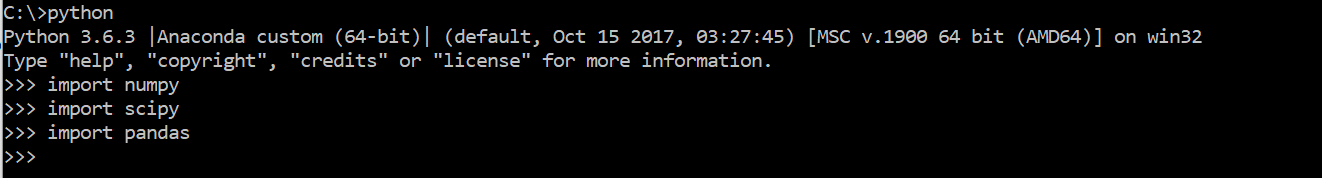
\includegraphics[width=0.8\textwidth]
    {figs/install/python_test.png} }
  \caption{Testing the Python environment.}
  \label{fig:python_test}
\end{figure}

%===============================================================================
\section{Set up your local SimCenter working environment}\label{setup}
%===============================================================================

To run the workflows locally, the backend of SimCenter desktop applications use publicly available software. These software need to be installed and configured on your operating system. If you do not plan to run the workflows locally, you will not need these applications.

\subsection{Set up OpenSees}
%===============================================================================

OpenSees is publicly available for download at its \href{https://opensees.berkeley.edu/OpenSees/user/download.php}{website}. You need to register your e-mail to gain access (\autoref{fig:opensees_register}). After registration, you can log in and download OpenSees and the corresponding Tcl version. 

Follow the instructions at the website to install Tcl (\autoref{fig:opensees_installation}). On Windows, make sure you run the installer as administrator, otherwise you will not be able to create the \texttt{C:/Program Files/Tcl} folder.

After Tcl is installed, we recommend you to put OpenSees in the \texttt{C:/SimCenter/OpenSees} folder on Windows and in the \texttt{Documents/SimCenter/OpenSees} folder on Mac.

\begin{figure}[!htbp]
  \centering {
    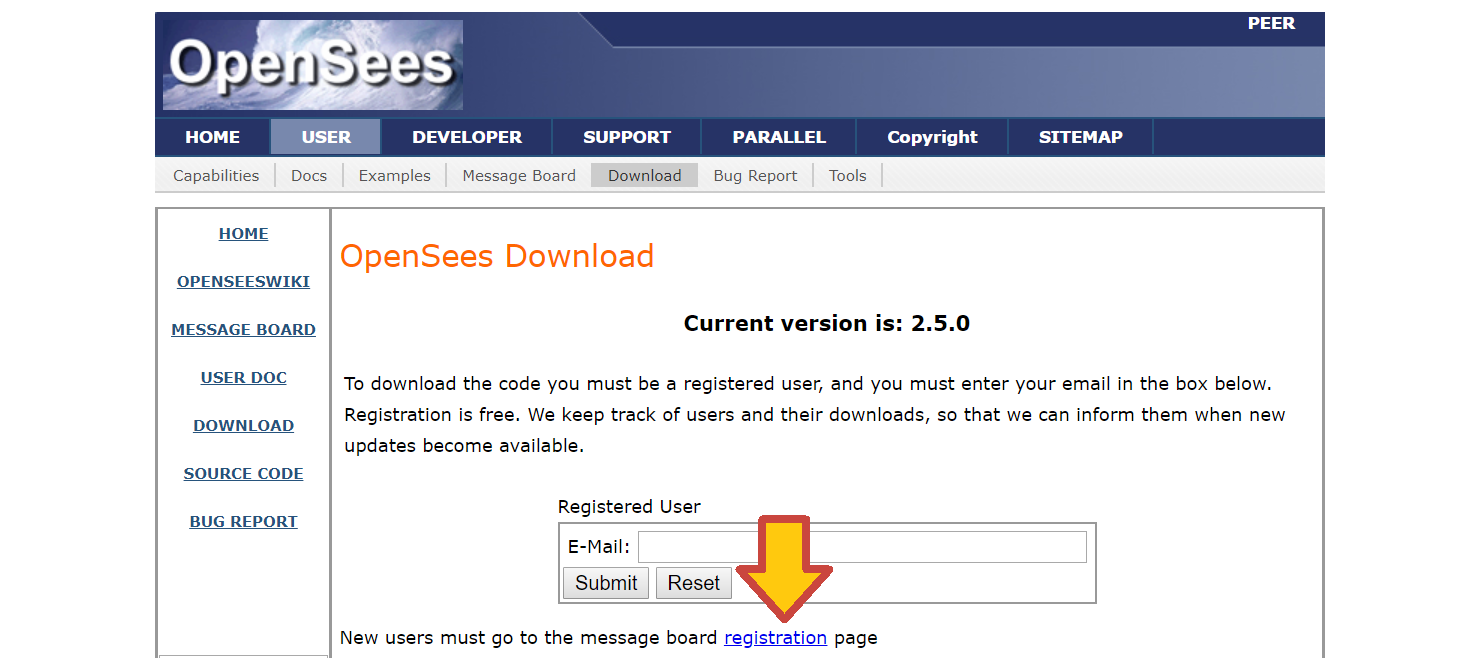
\includegraphics[width=0.8\textwidth]
    {figs/install/opensees_register.png} }
  \caption{Registration at the OpenSees website.}
  \label{fig:opensees_register}
\end{figure}

\begin{figure}[!htbp]
  \centering {
    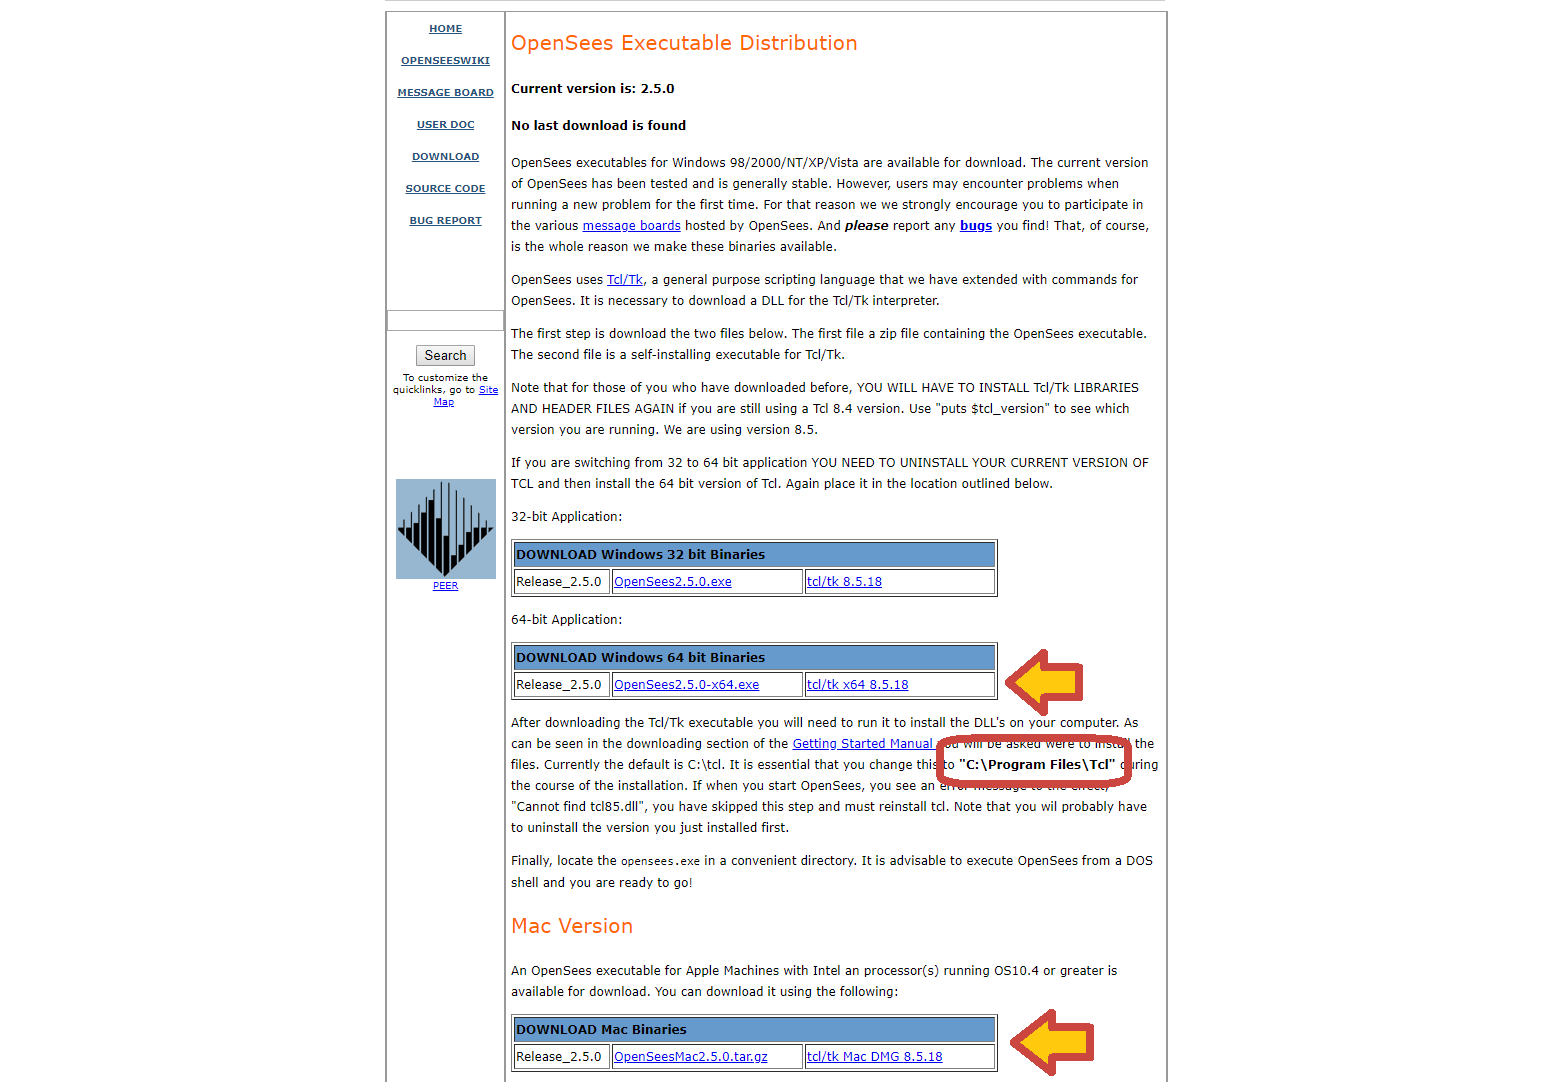
\includegraphics[width=0.8\textwidth]
    {figs/install/opensees_installation.png} }
  \caption{Installation instructions for OpenSees.}
  \label{fig:opensees_installation}
\end{figure}

You need to add the \texttt{OpenSees} folder to the system \texttt{PATH} environment variable to allow the SimCenter workflow applications to find the OpenSees executable on your computer. 

To add a folder to the \texttt{PATH} on Windows (\autoref{fig:add_env_path}):

\begin{itemize}
    \item open \emph{Start}, type \emph{env}, and choose \emph{Edit the system environment variables};
    \item click on the \emph{Environment variables...} button in the dialog window;
    \item find the \texttt{Path} under \emph{System Variables} in the \emph{Variable} column;
    \item click \emph{New} and type in the path to your \texttt{OpenSees.exe} (this will be \texttt{C:\\SimCenter\\OpenSees} if you put the executable at the recommended location - pay attention to using backward slashes here!);
    \item click \emph{OK} in every dialog to close them and save your changes.
\end{itemize}

\begin{figure}[!htbp]
  \centering {
    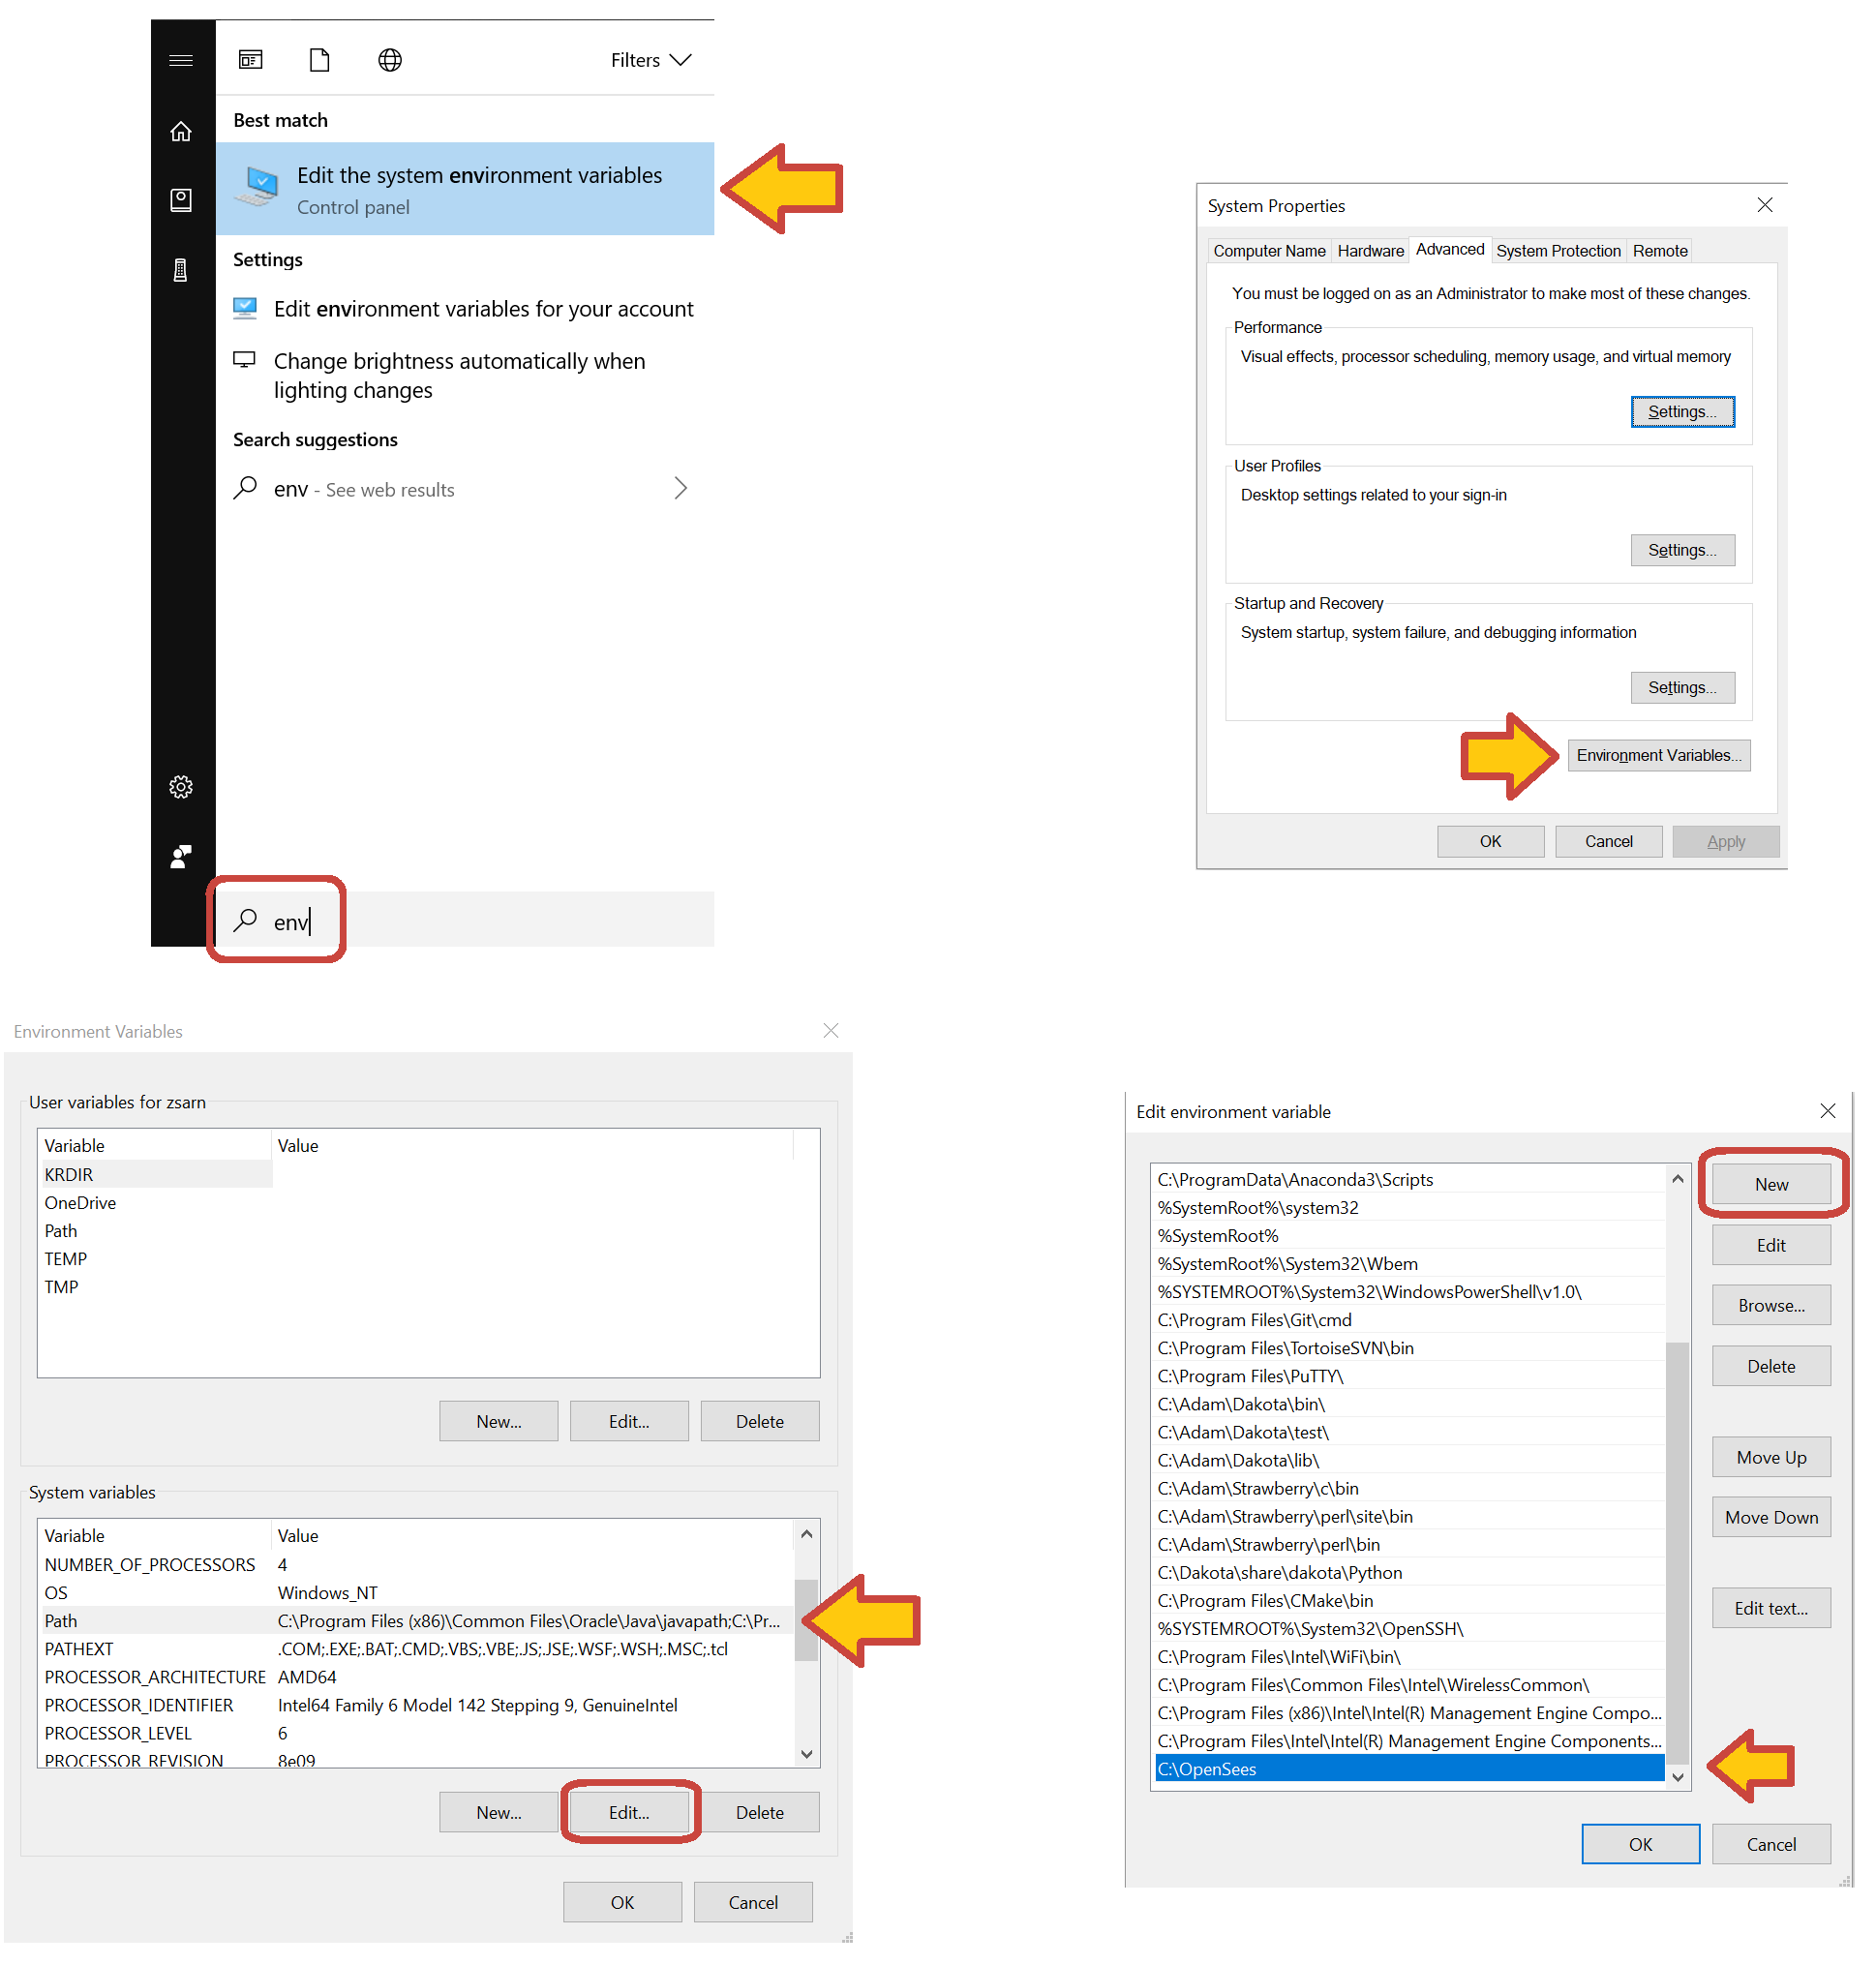
\includegraphics[width=0.8\textwidth]
    {figs/install/add_env_path.png} }
  \caption{Adding OpenSees to the PATH environment variable on Windows.}
  \label{fig:add_env_path}
\end{figure}

To add a folder to the \texttt{PATH} on Mac (\autoref{fig:add_env_path_Mac}):

\begin{itemize}
    \item open a Terminal;
    \item execute \texttt{sudo nano /etc/paths} and enter your password
    \item add the path to the OpenSees executable to the end of the list (this will be \texttt{/usr/Documents/SimCenter/OpenSees} if you put the executable at the recommended location);
    \item quit by hitting \texttt{Ctrl+X} and then \texttt{Y} when asked if you want to save modifications.
\end{itemize}

\begin{figure}[!htbp]
  \centering {
    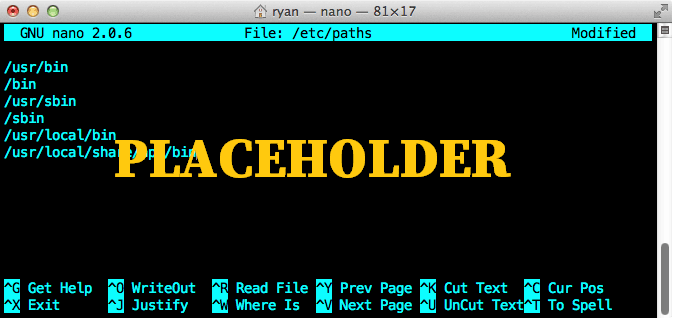
\includegraphics[width=0.8\textwidth]
    {figs/install/add_env_path_Mac.png} }
  \caption{Adding OpenSees to the PATH environment variable on Mac.}
  \label{fig:add_env_path_Mac}
\end{figure}

\subsection{Set up Dakota}
%===============================================================================

Dakota is publicly available for download at its \href{http://dakota.sandia.gov/download.html}{website}. Select your operating system from the list and set the other options according to \autoref{fig:dakota_installation}. Download the release in a \texttt{ZIP} file for Windows and \texttt{TAR.GZ} file for Mac. We recommend you to extract the archive to a \texttt{C:/SimCenter/Dakota} folder on Windows, and to a \texttt{Documents/SimCenter/Dakota} folder on a Mac.

\begin{figure}[!htbp]
  \centering {
    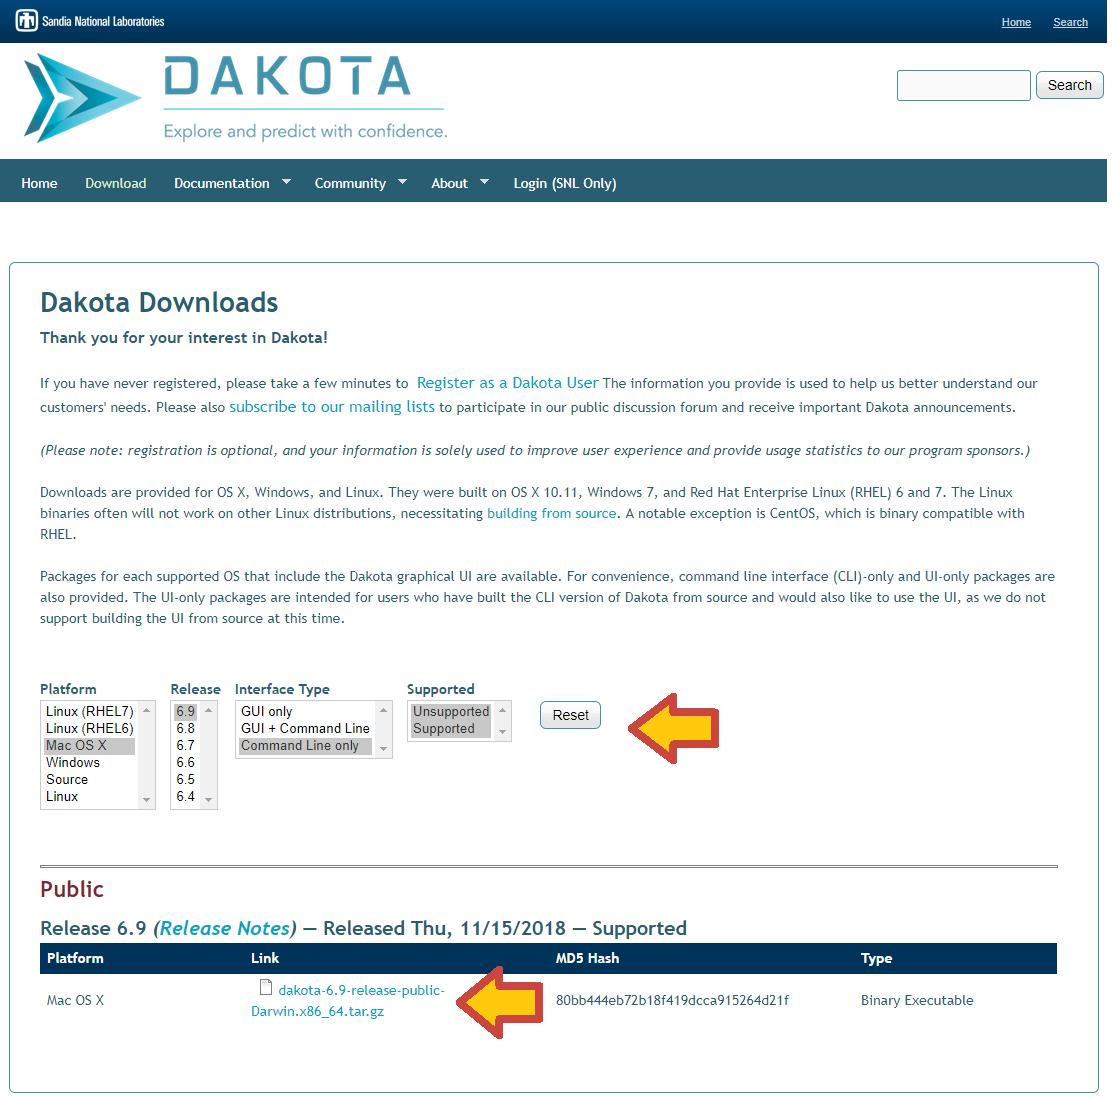
\includegraphics[width=0.8\textwidth]
    {figs/install/dakota_installation.png} }
  \caption{Adding OpenSees to the PATH environment variable on Mac.}
  \label{fig:dakota_installation}
\end{figure}

Similarly to OpenSees, you need to add the Dakota folders to the system \texttt{PATH} environment variable to allow the SimCenter workflow applications to find the Dakota tools on your computer. Use the procedure described above for OpenSees to add the following folders to your \texttt{PATH}:

On Windows:
\begin{itemize}
    \item \texttt{C:\textbackslash SimCenter\textbackslash Dakota\textbackslash bin}
    \item \texttt{C:\textbackslash SimCenter\textbackslash Dakota\textbackslash share\textbackslash dakota\textbackslash Python}
\end{itemize}

On Mac:
\begin{itemize}
    \item \texttt{/usr/Documents/SimCenter/Dakota/bin}
    \item \texttt{/usr/Documents/SimCenter/Dakota/share/dakota/Python}
\end{itemize}

\subsection{Set up Perl}
%===============================================================================

Mac OS X has Perl pre-installed, but Windows users will have to install it to be able to use every functionality in Dakota. We recommend you to use Strawberry Perl; you can install it by downloading the executable from its \href{http://strawberryperl.com}{website} and running it.

\subsection{Test the local applications}
%===============================================================================

Before running the EE-UQ application, perform the following tests to make sure that the local SimCenter working environment is set up appropriately:

\begin{itemize}
    \item Start a Terminal on Mac or a Command Prompt on Windows.
    \item On Mac, execute \texttt{cd /usr/Documents} to change the active directory to \texttt{/usr/Documents}. On Windows, execute \texttt{cd C:/} to change the active directory to \texttt{C:/}.
    \item Test if OpenSees works correctly by executing the \texttt{OpenSees} command. The command should start OpenSees (\autoref{fig:opensees_test}). Close OpenSees with the \texttt{exit} command.
    \item Test if Dakota works correctly by executing the \texttt{dakota} command. The command should start Dakota and you should see a message about a missing argument (\autoref{fig:dakota_test}).
    \item Test if Perl works correctly by executing the \texttt{perl -v} command. The command should start Perl and return its version number (\autoref{fig:perl_test}).
    \item Test if the python package in Dakota works correctly by starting Python with the \texttt{python} command and then executing the \texttt{import dakota} command. This should import the dakota package. If you do not see errors, then the package is successfully imported (\autoref{fig:dakota_py_test}). Exit Python with the \texttt{exit()} command.
    \item If all the above tests ran without errors, your environment is set up appropriately.
\end{itemize}

\begin{figure}[!htbp]
  \centering {
    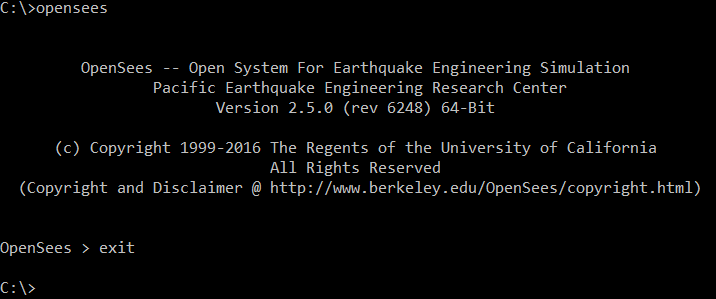
\includegraphics[width=0.8\textwidth]
    {figs/install/opensees_test.png} }
  \caption{Testing OpenSees.}
  \label{fig:opensees_test}
\end{figure}

\begin{figure}[!htbp]
  \centering {
    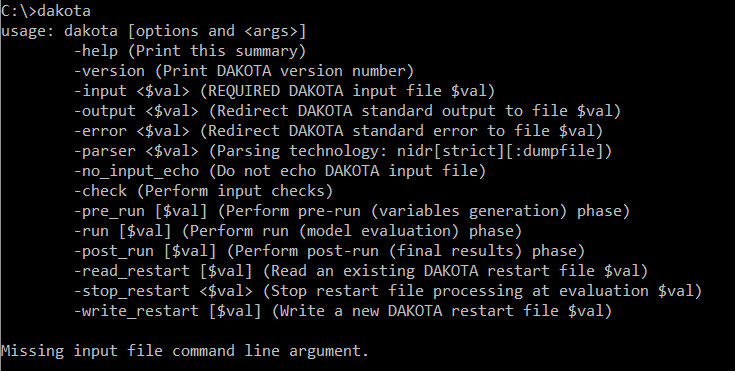
\includegraphics[width=0.8\textwidth]
    {figs/install/dakota_test.png} }
  \caption{Testing Dakota.}
  \label{fig:dakota_test}
\end{figure}

\begin{figure}[!htbp]
  \centering {
    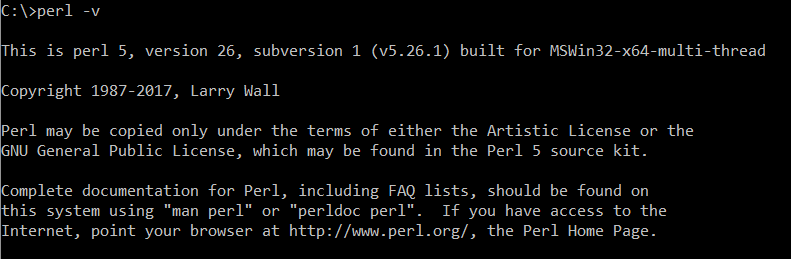
\includegraphics[width=0.8\textwidth]
    {figs/install/perl_test.png} }
  \caption{Testing Perl.}
  \label{fig:perl_test}
\end{figure}

\begin{figure}[!htbp]
  \centering {
    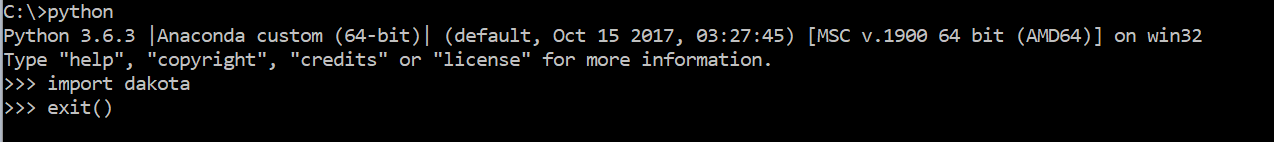
\includegraphics[width=0.8\textwidth]
    {figs/install/dakota_py_test.png} }
  \caption{Testing the dakota Python package.}
  \label{fig:dakota_py_test}
\end{figure}

%===============================================================================
\section{Test the EE-UQ application}\label{install_test}
%===============================================================================

\subsection{Run a remote calculation}
%===============================================================================

\subsection{Run a local calculation}
%===============================================================================

